% Criterion 4: Students
% Updated from the authoritative DOCX dated 02-08-2026.
% Required packages in the main document:
%   graphicx, float, booktabs, array, multirow, hyperref
% Qalam evidence images are included conditionally when criterion4_assets is available.

\chapter{Criterion 4: Students}
\label{criterion4}

The success of the BESE program at NUST-SEECS is evaluated through the quality of admitted students, their academic progress, and the effectiveness of student support and quality assurance processes. The institute provides academic guidance, monitors progress towards program goals, and regularly reviews its procedures to maintain high standards. NUST-SEECS also promotes ethical values, interpersonal skills, and student well-being through sports, clubs, societies, professional chapters, and other co- and extracurricular activities. Admission is managed centrally by the NUST Admissions Directorate. Applicants must meet PEC eligibility requirements and take a competitive entrance examination. Merit is determined by performance in the admission examination and previous academic record, along with the applicant's stated program preferences.

\section{Eligibility Criteria and Admission Requirements}
\label{sec:admission-criteria}

Admission to the BE Software Engineering (BESE) programme at NUST-SEECS is
governed by NUST's undergraduate admission policy
(NUST Undergraduate Prospectus 2025)\footnote{NUST Undergraduate Prospectus 2025,
\url{https://nust.edu.pk/wp-content/uploads/2020/03/MARCOMS-PROSPECTUS-2025-V.5.0-04032025_compressed.pdf}.
The prospectus for the respective admission year applies to each batch.}
and the minimum eligibility requirements prescribed by the Pakistan Engineering
Council (PEC). The admission process ensures that candidates meet the prescribed
academic qualifications, possess an eligible subject background, and satisfy the
university's merit-based selection criteria. The principal eligibility
requirements are summarized in Table~\ref{tab:admission-eligibility}.

\begin{table}[htbp]
\centering
\caption{Eligibility Criteria for Admission to BE Software Engineering}
\label{tab:admission-eligibility}
\small
\renewcommand{\arraystretch}{1.2}
\begin{tabular}{|p{0.25\textwidth}|p{0.67\textwidth}|}
\hline
\textbf{Requirement} & \textbf{Eligibility Criteria} \\ \hline
SSC / Matriculation & Minimum 60\% aggregate marks or equivalent. \\ \hline
HSSC / Intermediate & Minimum 60\% aggregate marks or equivalent, with an accepted subject combination. \\ \hline
Pre-Engineering & Mathematics, Physics, and Chemistry. \\ \hline
ICS / Computer Science & Mathematics, Physics and Computer Science; eligible for all Engineering programmes subject to clearing Chemistry as a remedial course in the first semester. \\ \hline
Pre-Medical & Eligible for Engineering programmes either by passing NUST’s additional Mathematics exam, or by completing NUST’s 8-week condensed Mathematics course prior to admission. \\ \hline
O/A Levels or foreign qualifications & Relevant IBCC equivalence certificates demonstrating compliance with the prescribed subject and minimum-mark requirements. \\ \hline
Admission test and merit & Participation in the applicable NUST Entry Test (NET) and fulfilment of the university's merit-based selection criteria. \\ \hline
\end{tabular}
\end{table}

Candidates must hold at least 60\% aggregate marks in SSC and HSSC (or equivalent). FSc candidates may apply on FSc Part-I marks, with admission confirmed on submission of the FSc certificate or Detailed Marks Certificate showing at least 60\% aggregate. Candidates with an HSSC Pre-Engineering background must have studied Mathematics, Physics, and Chemistry. Candidates with an ICS/Computer Science background must have studied Mathematics, Physics, and Computer Science and are required to clear Chemistry as a remedial subject in the first semester, in accordance with the applicable policy. Eligible candidates from the Pre-Medical group may apply subject to fulfilment of NUST's prescribed condensed Mathematics requirements. Candidates holding O/A Level or other foreign qualifications must provide the relevant equivalence certificates issued by the Inter Board Committee of Chairmen (IBCC), demonstrating compliance with the prescribed subject and minimum-mark requirements. Admission is merit-based and processed through the NUST Entry Test (NET) and the university's prescribed selection procedure. The process is managed centrally by the NUST Admissions Directorate, which applies the approved eligibility criteria and merit determination procedure, as summarized in Table~\ref{tab:admission-merit}.

\begin{table}[H]
\centering
\caption{Admission Category Percentage}
\label{tab:admission-merit}
\begin{tabular}{@{}lc@{}}
\toprule
\textbf{Category} & \textbf{Percentage} \\
\midrule
NUST Entry Test & 75\% \\
HSSC / A Level / Equivalent / DAE or HSSC Part-I & 15\% \\
Matriculation / O Level\textsuperscript{*} & 10\% \\
\bottomrule
\end{tabular}
\vspace{0.4em}
\begin{minipage}{0.92\textwidth}
\footnotesize
\textsuperscript{*}O/A Level final-year candidates are assigned 25\% to O Level equivalence as per the IBCC certificate.
\end{minipage}
\end{table}

Compliance with PEC's minimum admission requirements is supported by the published admission policy, verification of candidates' academic qualifications and subject combinations, NET results, merit lists, IBCC equivalence certificates, and records of remedial-course completion, where applicable. These measures promote transparent admissions and provide documentary evidence for assessing compliance with the applicable PEC requirements. 

\section{Annual Intake and Admission Response}
\label{sec:annual-intake}
The programme's annual intake is also considered in relation to its approved capacity and available academic resources. The annual student intake, admission response, and current enrollment for batches 2K23, 2K24, 2K25, and 2K26, are outlined in Table~\ref{tab:annual-intake}. %, which can also be found in \hyperref[annex:D1]{Annex D1}.

%\begin{table}[htbp]
%\centering
%\caption{Annual Intake and Admission Response}
%\label{tab:annual-intake}

%\normalsize
%\renewcommand{\arraystretch}{1.25}
%\setlength{\tabcolsep}{9pt}

%\begin{tabular}{lccc}
%\toprule

%\textbf{Intake Batch} &
%\makecell[c]{\textbf{Intake}\\
%             \textbf{(Allowed / Present)}} &
%\makecell[c]{\textbf{No. of Applicants}\\
%             \textbf{(/ Acceptance Rate)}} &
%\textbf{Sections} \\

%\midrule

%Fall 2023 & 90 / 88 & 14,525 / 0.6\% & 2 \\
%Fall 2024 & 90 / 88 & 12,084 / 0.7\% & 2 \\
%Fall 2025 & 90 / 87 & 13,522 / 0.6\% & 2 \\
%Fall 2026 & 90 / 88 & 15,124 / 0.6\% & 2 \\
%\midrule

%\textbf{Total} &
%\textbf{360 / 351} &
%-- &
%\textbf{8} \\

%\bottomrule
%\end{tabular}
%\end{table}

\begin{table}[htbp]
\centering
\caption{Annual Intake and Admission Response}
\label{tab:annual-intake}
\small
\begin{tabular}{c l c c c c c}
\toprule
\textbf{\makecell{Sr.\\No.}} &
\textbf{\makecell[l]{Intake\\Batch}} &
\textbf{\makecell{Total\\Applicants}} &
\textbf{\makecell{Total Admissions\\Offered$^{*}$}} &
\textbf{\makecell{Acceptance\\Rate (\%)}} &
\textbf{\makecell{Present\\Strength}} &
\textbf{\makecell{No. of\\Section(s)}} \\
\midrule
1 & Fall 2023 & 14525 & 90 & 0.61\% & 85  & 2 \\
2 & Fall 2024 & 12084 & 90 & 0.74\% & 88  & 2 \\
3 & Fall 2025 & 13522 & 90 & 0.66\% & 88  & 2 \\
4 & Fall 2026 & 15124 & 90 & 0.59\% & 88  & 2 \\
\midrule
 & \textbf{Total} & \textbf{55255} & \textbf{360} & -- & \textbf{349} & -- \\
\bottomrule
\end{tabular}

\vspace{2pt}
\begin{flushleft}
\footnotesize $^{*}$ Total admissions offered in all the merit lists.
\end{flushleft}
\end{table}

%\section{Policy \& Processes for Transfer/Migration }
%\label{sec:student-transfer}

%Transfers are considered only on justifiable grounds and with approval of the Rector on the recommendation of the Principal, in accordance with NUST, HEC, and PEC regulations. The existing NUST policy permits migration after completion of the first year and before the final year; requires an academic record comparable with NUST admission standards; and, for transfers from another institution, requires a No Objection Certificate and a good-character/disciplinary-status certificate. Internal migration is restricted to students admitted through the NUST Entry Test.

\phantomsection
\section{Policies and Processes for Credit Transfer and Exemption}
\label{app:criteria3-credit-transfer}

NUST regulates credit transfer through two policies: the \textit{Migration and Transfer Policy}\footnote{Policy Code 26-00-005-04, approved 22 December 2021} and the \textit{Policy on Change of UG Program/Disciplines} (Annexure~\ref{annex:D1}). Both are administered by the Registrar Directorate, with academic evaluation carried out by the concerned school or college.

\subsection{Eligibility of Courses}
Credit is granted only for courses that satisfy the following conditions:
\begin{itemize}
    \item The student has earned at least a \textbf{B grade} in the course.
    \item The course corresponds to a NUST course, or is equivalent to one in depth and intensity.
    \item The student completes at least \textbf{60\%} of the credit hours of the degree programme at NUST.
\end{itemize}
Transferred credits count toward degree requirements, but their grades are \textbf{not} included in the CGPA calculation. Detailed requirements regarding parent institute, timeline, \% of CH, and NOC are outlined in Annexure~\ref{annex:D1}.

\subsection{Process}
\begin{enumerate}
    \item \textbf{Application:} The student submits the prescribed form with the official transcript, detailed course outlines, an NOC from the parent institution and the processing fee.
    \item \textbf{Course evaluation:} The receiving school or college evaluates the transcript and course outlines. It then lists the \textit{accepted courses} (with credits and grades) and the \textit{deficient courses} that the student must still complete.
    \item \textbf{Recommendation:} The Principal/Dean/Commandant recommends or rejects the case, and the Registrar Directorate processes it.
    \item \textbf{Approval:} The Rector approves migration cases, and the competent authority approves internal change-of-program cases.
\end{enumerate}

\subsection{Credit Treatment by Case}
\begin{table}[htbp]
\centering
\small
\begin{tabular}{p{3.6cm} p{9cm}}
\toprule
\textbf{Case} & \textbf{Credit Treatment} \\
\midrule
Migration from another institution & Accepted courses are credited after evaluation. Deficient courses must be completed at NUST. \\
Transfer within NUST & Allowed once only. Credits are evaluated by the receiving institute. \\
Change of program (first year common) & Accepted credits and grades are fully transferable. Leftover courses are recorded as non-credit additional courses, and the institute prepares a plan to make up any single deficient course. \\
Change of program (first year not common) & The student chooses Option~I (start afresh with no credit transfer) or Option~II (transfer of all accepted credits, with previous study time counted in the duration). Leftover courses are recorded as non-credit additional courses. \\
\bottomrule
\end{tabular}
\end{table}

\subsection{Related Conditions}
Students who migrate, or who change programs with credit transfer, are not eligible for honours and awards, except the Rector's Gold Medal. A change of program is allowed only once and cannot be reversed.

\begin{sloppypar}
Before acceptance, the required process evaluates course content, credit hours, grades, and learning outcomes for work completed in a PEC-accredited program of an HEC-recognized institution. No more than 50\% of the degree credit hours may be transferred, and each accepted transfer must be recorded and intimated to PEC at the time of acceptance. The transfer and migration policy is attached as Annexure~\ref{annex:D1}.
\end{sloppypar}


\section{Academic Counselling and Student Advisory System (SAS)}
\label{sec:sas}

%Each student is assigned a faculty advisor at the start of the program. The advisor serves as the student's first point of contact for academic matters, personal guidance, and professional development throughout the degree. The Student Advisory System (SAS) policy and related forms are provided in Annexure~\ref{annex:D2}.

%Students are organized into advisory groups of approximately 10--20 students. Several faculty members serve as Student Advisors under the supervision of the Department's Student Advisory Coordinator. The advisors monitor academic progress, attendance, conduct, and general well-being, and refer matters requiring specialized intervention to the relevant office. Advisory meetings are held several times every semester. Students with weak academic performance are counselled individually and may be directed towards coaching, tutoring, or other support. Records of advisory meetings and follow-up actions are maintained; representative records are provided in \hyperref[annex:D4]{Annex D4}.

%The advisory record is retained in Qalam and is visible to the relevant academic and administrative personnel. This provides transparency, traceability, and support for academic quality assurance.

Each critical student is supported by a faculty Student Advisor (SA) who serves as the first point of contact for academic matters, personal guidance and professional development. Advising is mandatory for all first-year students and for critical students, meaning those whose cumulative or semester GPA is below the qualifying grade or who have more than one F/XF/W grade. It is voluntary for other students, and the Head of Institution may add any student to the system. The Student Advisory System (SAS) policy and related forms are provided in Annexure~\ref{annex:D2}. 

Several faculty members serve as Student Advisors under the supervision of the Department's Student Advisory Coordinator. Critical students are assigned to dedicated advisors, with a maximum of 10 students per advisor. Advisor allocation for critical students identified in Fall 2026 are shown in Figure~\ref{fig:critical}. 

\begin{figure}[H]
\centering
\fbox{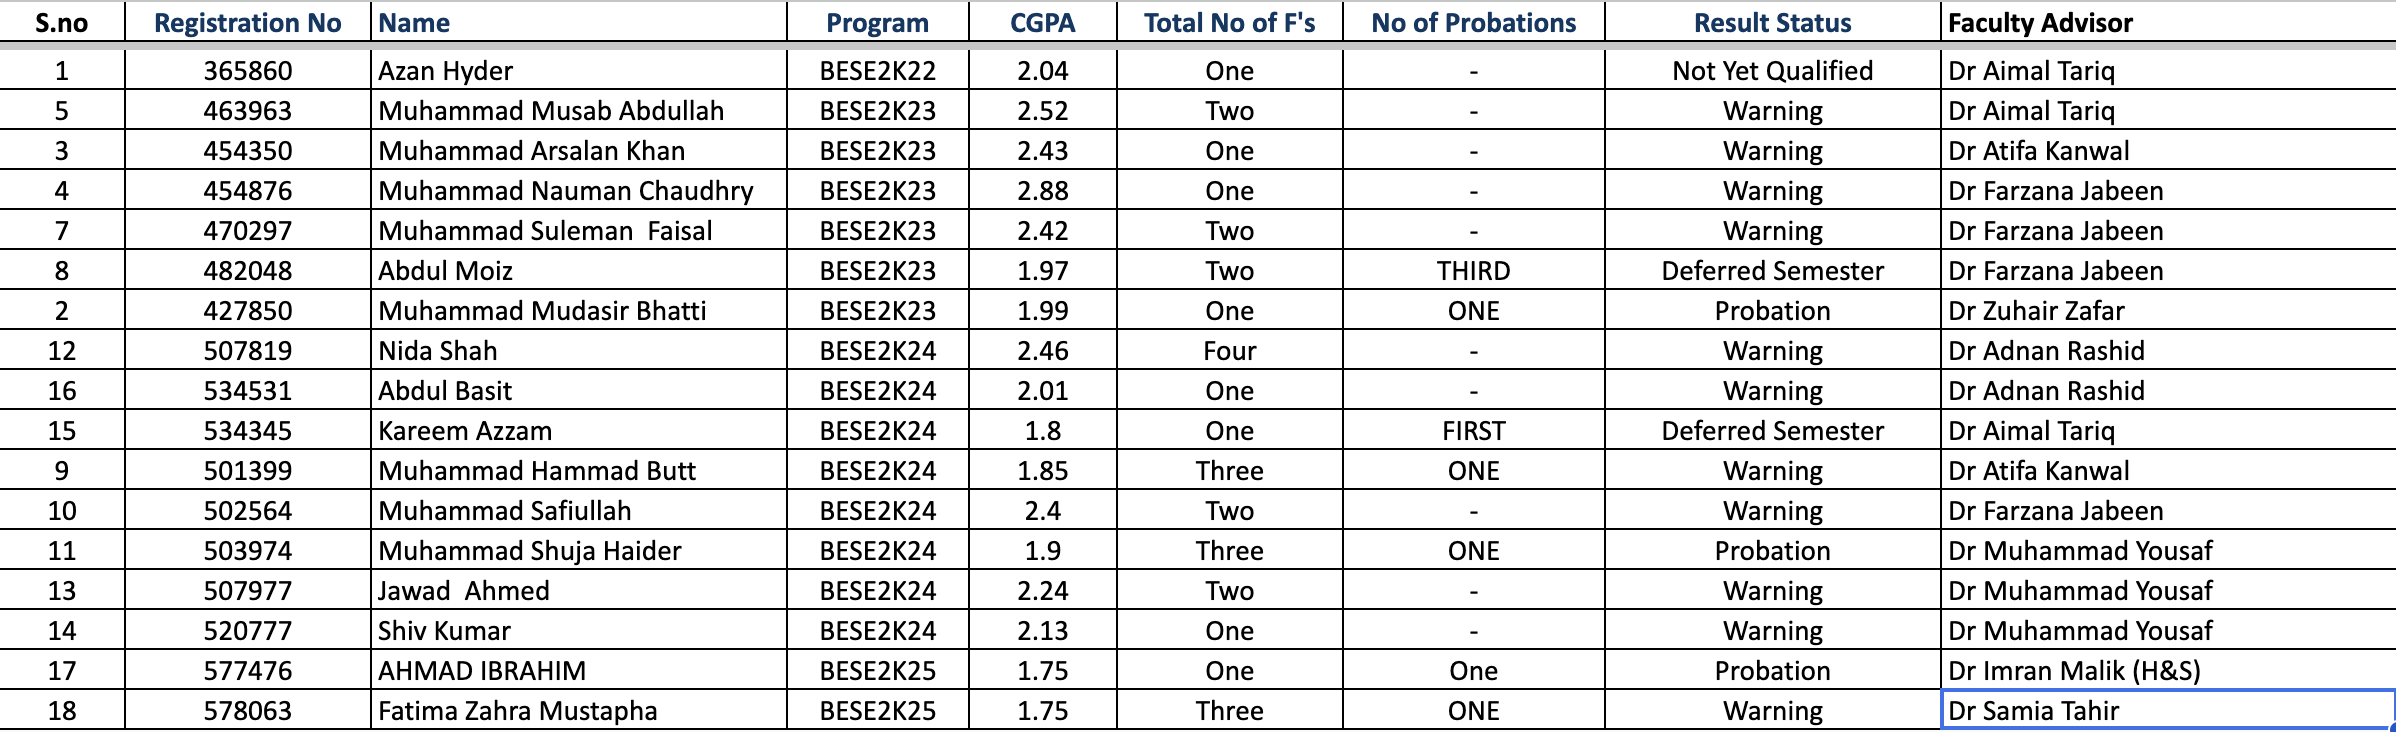
\includegraphics[width=1.0\textwidth]{images/criterion_4/critical.png}}
\caption{Advisor Allocation to Critical Students Identified in Fall 2026}
\label{fig:critical}
\end{figure}

The advisors monitor academic progress, attendance, conduct, and general well-being, and refer matters requiring specialized intervention to the relevant office. Parents are often contacted if required to keep them in the loop. Advisory meetings are held multiple times in each semester and are scheduled by the Academic Coordination Branch (ACB) (Figure~\ref{fig:schedule}). 

\begin{figure}[H]
\centering
\fbox{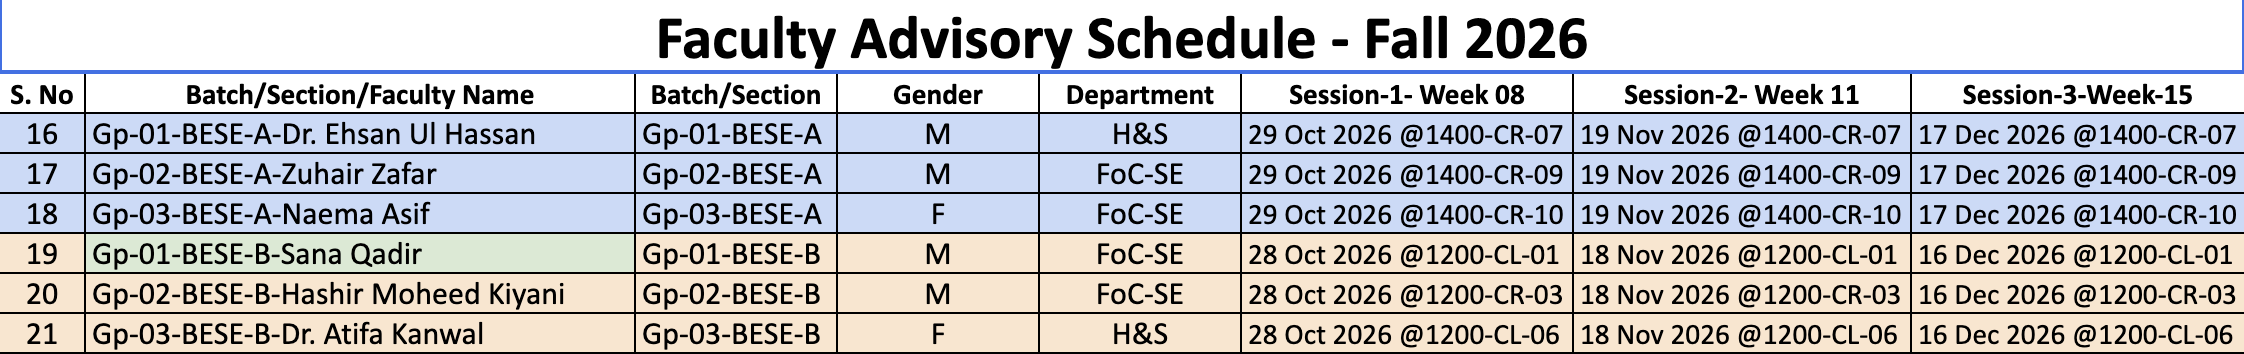
\includegraphics[width=1.0\textwidth]{images/criterion_4/schedule.png}}
\caption{Schedule for SAS Meetings in Fall 2026}
\label{fig:schedule}
\end{figure}

Students with weak academic performance are counselled individually and may be directed towards coaching, tutoring, or other support. Records of advisory meetings and follow-up actions are maintained (sample template for advisory record is presented in Annexure~\ref{annex:D3}). Reporting for critical students is automated in Qalam, which identifies them after results are announced, generates their academic progress sheets, supports advisor feedback reports and issues warning letters. 

\section{Career and Student Wellness Counselling}
\label{sec:career-wellness}

A formal orientation is conducted during the first week of each new batch to brief students on program requirements, academic regulations, support services, and professional expectations. The NUST Student Support Services Centre (S3C) serves as a one-window facilitation point. C3A provides professional counselling for academic, social, emotional, stress-related, and psychological concerns and conducts psychological assessments where appropriate. The Career Development Centre (CDC) supports career exploration, professional development, employer engagement, industry sessions, interviews, and recruitment drives. Further details are also discussed in subsequent chapters.


\section{Policies Dealing with Harassment \& Plagiarism}
\label{sec:plag}
\subsection{Academic Misconduct}
The NUST Code of Conduct (Undergraduate Student Handbook, Chapter~11) defines academic dishonesty as any act of fraud intended to influence a grade or academic evaluation. It covers cheating, fabrication, plagiarism, facilitating dishonesty and unauthorized collaboration. The use of unfair means, such as possessing unauthorized material or communicating with others during a test or examination, is also prohibited. Suspected cases are reported to the head of the institution through the Head of Department. The Institution Discipline Committee holds a hearing and gives the student a full opportunity to present his or her viewpoint before recommending a punishment. Penalties are proportional to the gravity of the case. Minor punishments include a written warning, probation, a fine of up to Rs~10,000, removal of privileges and the award of an F grade in the course. Major punishments include expulsion from class for up to one semester, a fine of up to Rs~50,000, cancellation of examination results, rustication, non-conferment of the degree and relegation or withdrawal. Minor punishments are awarded by the head of the institution, and major punishments for civilian students are awarded by the Rector on the recommendation of the NUST Discipline Committee. The student may appeal to the head of the institution or the Rector within fifteen days of the decision, and the parents of students who violate the Code are informed. Reference from UG Student Handbook is presented in Annexure~\ref{annex:D4} while complete handbook is available at SEECS Website\footnote{https://seecs.nust.edu.pk/wp-content/uploads/2024/09/28-Aug-2024-Undergraduate-Handbook.pdf}.
\subsection{Research-Related Plagiarism}
Research-related plagiarism and ethics cases are governed by the NUST Research Ethics and Plagiarism Policy\footnote{https://seecs.nust.edu.pk/wp-content/uploads/2020/06/Plagiarism-Policy-approved.pdf}, which complements the HEC Anti-Plagiarism Policy. The policy applies to all students, teachers, researchers and staff involved in research. Complaints are submitted to the Research Directorate with supporting evidence, and cases are heard by the NUST Standing Committee on Plagiarism and Research Ethics, chaired by the Pro-Rector (RIC). The committee works independently, members with a conflict of interest withdraw, the identities of those involved are kept confidential, and all parties are given a fair chance to present their case. Its decision is communicated to all stakeholders. All publications, theses and assignments are screened through Turnitin, and in line with HEC guidelines overall similarity must not exceed 19\% and similarity with any single source must not exceed 5\%.
\subsection{Zero-tolerance Policy on Harassment}
NUST follows a zero-tolerance policy on harassment\footnote{https://c3a.nust.edu.pk/wp-content/uploads/2020/11/NUST-Policy-on-Protection-Against-Harassment-6.pdf}, aligned with the Protection Against Harassment of Women at the Workplace (Amendment) Act 2022 and the HEC 2025 guidelines. The policy applies to students, faculty, staff and third parties, on campus, in NUST-recognized activities and online. Complaints may be informal (verbal or written, resolved by confidential mediation for lower-degree cases) or formal (written), and can be raised through focal persons, student advisors, supervisors, the HoD or Principal, any Inquiry Committee member or the anti-harassment helpline. Formal complaints go to a three-member Inquiry Committee that includes at least one woman. It informs the respondent within 3 working days, receives a reply within 7 working days, and submits its recommendations to the Rector within 30 working days. The Rector implements the decision within 7 working days. Proceedings are confidential, both parties are treated under the principles of natural justice, and complainant and respondent sign a non-contact undertaking. Reprisals are prohibited, and interim measures such as schedule changes or temporary suspension may be applied. Penalties follow the NUST statutes for students and employees, and malicious complaints are themselves punishable. Either party may appeal within 30 working days to a three-member Appellate Body or to the Ombudsman. NUST also runs awareness and sensitization training for focal persons and committee members.

\section{Semester Workload and Class Size}
\label{sec:class-size}
The program is divided into 8 semesters with course load each semester following the standards set by PEC and HEC. Table~\ref{tab:credit-hours} shows the breakdown of CHs for each semester of current BESE batches.

\begin{table}[H]
\centering
\caption{Credit hours breakdown for each semester for Batch 2k23, 2k24 and 2k25 \& onwards}
\label{tab:credit-hours}
\resizebox{\textwidth}{!}{%
\begin{tabular}{@{}crrrrrr@{}}
\toprule
\multirow{2}{*}{\textbf{Semester}} & \multicolumn{3}{c}{\textbf{Batch 2k23 and 2k24}} & \multicolumn{3}{c}{\textbf{Batch 2k25 \& onwards}} \\
\cmidrule(lr){2-4}\cmidrule(l){5-7}
& \textbf{CHs Teaching} & \textbf{CHs Labs} & \textbf{Total Credit Hours} & \textbf{CHs Teaching} & \textbf{CHs Labs} & \textbf{Total Credit Hours} \\
\midrule
1 & 16 & 2 & 18 & 14 & 4 & 18 \\
2 & 13 & 5 & 18 & 15 & 3 & 18 \\
3 & 15 & 3 & 18 & 15 & 3 & 18 \\
4 & 15 & 3 & 18 & 16 & 2 & 18 \\
5 & 14 & 4 & 18 & 14 & $3+X$ & $17+X$ \\
6 & 16 & $1+X$ & $17+X$ & 16 & $1+X$ & $17+X$ \\
7 & 11 & $2+X$ & $13+X$ & 12/13/14 & 5/4/3 & 17 \\
8 & 7 & 7 & 14 & 8/9/10 & 7/6/5 & 15 \\
\midrule
\multicolumn{3}{r}{\textbf{Grand Total}} & \textbf{$134+X$} & \multicolumn{2}{r}{\textbf{Grand Total}} & \textbf{$138+X$} \\
\bottomrule
\end{tabular}%
}
\end{table}
The class size for theory and practical sessions is the same. The class size and sample lab size of active batches of the BESE program is summarized in Table~\ref{tab:class-size} and Table~\ref{tab:lab-size} respectively.

\begin{table}[H]
\centering
\caption{Class Size of Current Batches}
\label{tab:class-size}
\begin{tabular}{@{}clrrrr@{}}
\toprule
\textbf{Sr. No.} & \textbf{Batch} & \textbf{Year of Intake} & \textbf{Size} & \textbf{No. of Sections} & \textbf{Average/Section} \\
\midrule
1 & BESE-14 & 2023 & 85 & 2 & 42.5 \\
2 & BESE-15 & 2024 & 88 & 2 & 44 \\
3 & BESE-16 & 2025 & 88 & 2 & 44 \\
4 & BESE-17 & 2026 & 88 & 2 & 44 \\
\bottomrule
\end{tabular}
\end{table}

\begin{table}[H]
\centering
\caption{Sample of Lab Size}
\label{tab:lab-size}
\begin{tabular}{@{}clcc@{}}
\toprule
\textbf{Sr. No.} &
\textbf{Lab} &
\textbf{Number of Workstations} &
\textbf{Workstations per Student} \\
\midrule
1 & Computing Lab 4 & 45 & 1 \\
2 & Computing Lab 5 & 45 & 1 \\
\bottomrule
\end{tabular}
\end{table}

\section{Completion of Courses and Student Feedback}
\label{sec:course-feedback}

Student feedback is collected twice during each semester, once before the MSE and again before the ESE. At the end of each feedback cycle, faculty members whose feedback scores fall below 70\% are requested to meet with the HoD to discuss student concerns and identify measures to improve the overall learning experience. At the end of each course, students also give their feedback on the course through the Students Course Review Report. The student feedback report about the faculty is attached as Annexure~\ref{annex:D5}.

\section{Student Co- \& Extra Curricular Activities}
\label{sec:competitions}
NUST-SEECS circulates opportunities and encourages participation in various student clubs and societies. While students can join any club and society across NUST\footnote{https://sa.nust.edu.pk/directory/}, there are a list of clubs and societies initiated by SEECS students and faculty sponsors. These are listed below:

\begin{itemize}
    \item{Hack Club}
    \item{Entrepreneurs Club}
    \item{IEEE Chapter}
    \item{ACM Chapter}
    \item{Google Developers Chapter}
    \item{Game Developement Club}
    \item{Fitness Club}
    \item{Excursion Club}
\end{itemize}

Aside from the clubs and societies, students are facilitated and mentored by the faculty and the administrative staff to participate in various high impact national and international events. Recent examples in the existing record include SEECS and SE student participation in following prominant events:
\begin{itemize}
    \item Efabless AI Generated Design Contest,
    \item IMechE UAS Design Challenge Pakistan,
    \item Huawei ICT Competition,
    \item SOFTEC, the Kibo Robot Programming Challenge, and
    \item Finding Innovative \& Creative Solutions for Society (FICS)
\end{itemize}
The list of prominent participantions in various international/national competitions and exhibitions with in the last three years is provided in Annexure~\ref{annex:D6} while details will be provided in Evidence folder.

\subsection{Annual Sports Gala}
\label{subsec:sports-gala}

NUST/SEECS provides indoor and outdoor sports opportunities and conducts an annual Sports Gala involving undergraduate and postgraduate students as well as faculty. Activities include cricket, football, basketball, volleyball, table tennis, badminton, tennis, squash, athletics and tug of war.

\subsection{International Exposure}
\label{subsec:financial-support}

The NUST International Office also circulates semester-exchange opportunities through SEECS focal persons. The list of universities hosting NUST students for semester exchange is attached as Annexure~\ref{annex:D11}. SEECS and SE students have been availing these opportunities frequently. Example of recent student exchanges is given in Table~\ref{tab:exchange}. Further details are provided in Evidence folder.

\begin{table}[H]
\centering
\caption{Recent SE Student Semester Exchanges Under UGRAD Program}
\label{tab:exchange}
\begin{tabular}{@{}clcc@{}}
\toprule
\textbf{Sr. No.} &
\textbf{Student Name} &
\textbf{Semester} &
\textbf{University} \\
\midrule
1 & Aryan Zia & Spring 2026 & Sungkyunkwan University, South Korea \\
2 & Eisha Tur Raazia & Spring 2026 & Sungkyunkwan University, South Korea \\
\bottomrule
\end{tabular}
\end{table}

\subsection{Community Service Learning}
\label{sec:community-service}

Community Service Learning course (CSL-402) was introduced in Spring 2013 as an optional course for undergraduate and postgraduate students and was later made compulsory for final-year undergraduate students. It aims to develop civic sense, social responsibility, community engagement, and an understanding of social issues. The course carries 0--1 credit hour and includes six workshops covering community needs assessment, project planning, teamwork, communication, social responsibility, and reflective learning. Students complete at least 30 hours of community service; some activities may be performed on campus, while the remaining work is completed through approved philanthropic or community organizations under the guidance of a faculty advisor. The Spring 2025 course outline is provided in Annexure~\ref{annex:D7}.

\section{Student Performance Evaluation}
\label{sec:performance-evaluation}

Students are evaluated through assignments, quizzes, term projects, laboratories, the Mid Semester Examination (MSE), and the End Semester Examination (ESE). A typical distribution of marks is given in Table~\ref{tab:evaluation-distribution}.

\begin{table}[H]
\footnotesize
\centering
\caption{Typical Student Performance Evaluation}
\label{tab:evaluation-distribution}
\resizebox{0.8\textwidth}{!}{%
\begin{tabular}{@{}lclc@{}}
\toprule
\multicolumn{2}{c}{\textbf{Lab-based Course (3+1)\textsuperscript{*}}} & \multicolumn{2}{c}{\textbf{Non-Lab-based Course (3+0)}} \\
\cmidrule(lr){1-2}\cmidrule(l){3-4}
\textbf{Assessment Type} & \textbf{Percentage} & \textbf{Assessment Type} & \textbf{Percentage} \\
\midrule
\multicolumn{2}{l}{\textbf{Lab Theory (75\%)}} & & \\
Quizzes & 10--15\% & Quizzes & 10--15\% \\
Assignments & 5--10\% & Assignments & 5--10\% \\
Mid Semester Exam & 25--35\% & Mid Semester Exam & 25--35\% \\
Semester Project & 0--20\% & Semester Project & 0--20\% \\
End Semester Exam & 40--50\% & End Semester Exam & 40--50\% \\
\addlinespace
\multicolumn{2}{l}{\textbf{Lab (25\%)}} & & \\
Lab Work & 50--70\% & & \\
Lab Project & 10--20\% & & \\
Lab Final & 20--30\% & & \\
\bottomrule
\end{tabular}%
}
\end{table}

Most of these assessments are mapped to course CLOs. At the end of the semester, a comprehensive report is generated for each student, which demonstrates an accurate assessment of students' progress with respect to fulfilment of course CLOs, in a direct manner. The relative grading system uses A, B+, B, C+, C, D+, D, and F grades. An I grade is awarded when a student is absent from the final examination; a retest requires approval from the FBS. An XF grade is awarded where attendance is below 75\%. A failed course may be repeated in the summer semester or when next offered. The course instructor submits results to the HoD for consideration by the DBS. The results are then presented to the FBS, chaired by the Principal SEECS and attended by representatives of the NUST Examination Branch, for approval.

\section{KPI of Students Performance in Relation to PLOs}
\label{sec:kpi-plo}

The suitability and affectivity of the teaching methodology and assessment methods are checked by reviewing the overall PLO results of a course. In case the PLOs are not achieved or have low direct and indirect assessment results, the LQEC recommends appropriate action. Details are discussed in subsequent chapters. For a cohort level issue, instructor is asked to review the teaching and assessment methodology and suggest an action for improvement. The PEOs, PLOs and CLOs of the program and their mapping are explained in detail in previous chapters.

\section{Financial Support}
\label{sec:fin}
Students can avail financial assistance via performance-merit awards, NUST need-based/Trust Fund assistance, Honhaar/HEC, and provincial scholarships, PEC need-cum-merit support, fee deferment, and Ihsan Trust interest-free loans. Sample list of students currently receiving financial support is attached as Annexure~\ref{annex:D10}.



